\section{Introduction} \label{sec:intro}
There are a great many natural phenomena which involve the diffusion of small particles through solids; interface problems, such as the growth of a titanium dioxide layer on the surface of titanium metal exposed to air, are good examples~\cite{tegner2015high}.
If we wish to answer questions such as why these interfaces grow, or how quickly, we really need to understand how particles diffuse through crystal lattices, especially in the case when they interact with each other.
In this paper we will introduce a very simple locally interacting exclusion model of this kind of diffusion, and we will explore the continuum-level implications of such a model.

We would intuitively expect that our titanium interface growth problem would involve the diffusion of oxygen atoms through titanium metal crystals. Once the concentration of oxygen is high enough, the medium becomes titanium dioxide.
The oxygen atoms do this primarily by hopping between the interstitial sites between the titanium atoms.
% Need citation
It is extremely energetically unfavourable for multiple oxygen atoms to occupy such a site,
%citation needed
therefore to a good approximation we may regard these oxygen atoms as excluding each other from these sites, just like in ASEP~\cite{sugden2007dynamically, liggett1985interacting}.

Next, let us assume that the lattice that the oxygen atoms move through is fairly rigid\footnote{I.e. that the titanium atoms are quite tightly bound and don't move that much, which is reasonable as they are metal atoms in a metal.},
and that the interactions between the oxygen atoms are quite short-ranged\footnote{Any electrostatic forces should be rapidly screened by the metal, thus the main interaction should be via short-range electrostatics and electron sea distortion.}.
Finally, we should note that even though a problem like interface growth happens in three-dimensional space, the problem is rotationally and translationally invariant in a plane perpendicular to the direction of growth; therefore the
interesting aspects of the problem are one-dimensional. Indeed, in anisotropic solids it is often the case that diffusion occurs much more rapidly along parallel chains than in other directions.

Putting these assumptions together, we are motivated to investigate the model described by the rates detailed in Figure~\ref{fig:rates}. It is essentially the symmetric exclusion model, only now the presence of an adjacent particle
causes the hopping rate to change. We will henceforth refer to the model as the ``sticky hopping model'', or SHM.
\begin{figure}[h!]
\vspace{1em}
\label{fig:rates}
 \begin{tabular}{c@{\hspace{1em}}c@{\hspace{1em}}c@{\hspace{1em}}c}
    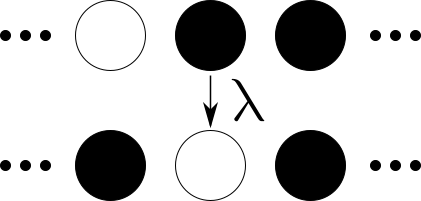
\includegraphics[width=0.22\linewidth]{../tex-src/images/rates4} & 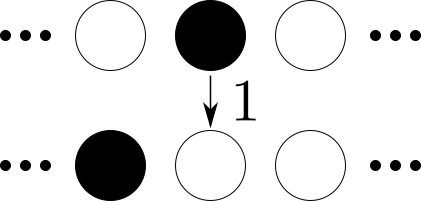
\includegraphics[width=0.22\linewidth]{../tex-src/images/rates1} & 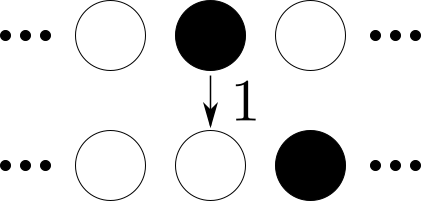
\includegraphics[width=0.22\linewidth]{../tex-src/images/rates2} & 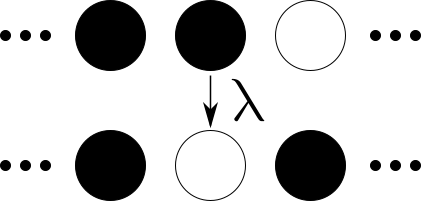
\includegraphics[width=0.22\linewidth]{../tex-src/images/rates3} \\
    \end{tabular}
    \vspace{-1em}
\caption{Filled circles indicate particles, empty circles indicate empty sites (vacancies). Particles randomly move into adjacent vacancies with rate $1$ (having rescaled time for notational convenience), unless there is a particle behind the position they're moving from,
in which case they move with rate $\lambda$; $\lambda<1$ represents attractive forces between particles, and $\lambda>1$ repulsive.}
\end{figure}
